\documentclass[showpacs,groupedaddress,showkeys,preprintnumbers]{revtex4-1}

\usepackage[colorlinks]{hyperref}
\usepackage{epstopdf}
\usepackage{amsmath}
\usepackage{stmaryrd} % For \shortuparrow and \shortdownarrow
\usepackage{upgreek} % For \upmu, upright mu

\newcommand{\be}{\begin{equation}}
\newcommand{\ee}{\end{equation}}
\newcommand{\ben}{$$}
\newcommand{\een}{$$}
\newcommand{\bea}{\begin{eqnarray}}
\newcommand{\eea}{\end{eqnarray}}
\newcommand{\bean}{\begin{eqnarray*}}
\newcommand{\eean}{\end{eqnarray*}}
\newcommand{\e}{{\rm e}}
\newcommand{\tr}{{\rm tr}}
\newcommand{\erf}{{\rm erf}}
\newcommand{\ie}{{\rm i.e.}}
\newcommand{\n}[1]{\label{#1}}
\newcommand{\ind}[1]{\mbox{\tiny{#1}}}
\newcommand{\nn}{\nonumber \\ \nonumber \\}
\newcommand{\Fp}{{\vec{F}}^{+}}
\newcommand{\Fc}{{\vec{F}}^{\times}}
\newcommand{\Vp}{{\vec{V}}^{+}}
\newcommand{\Vc}{{\vec{V}}^{\times}}
\newcommand{\abs}[1]{\lvert#1\rvert}
\newcommand{\norm}[1]{\lVert#1\rVert}
%\renewcommand{\vec}[1]{\mbox{\boldmath$#1$}}

% Graham's macros
\renewcommand{\vec}[1]{\mathbf{#1}}
\newcommand{\tran}[1]{ #1^{\rm T}}
%\newcommand{\abs}[1]{\left\vert#1\right\vert}
\newcommand{\fp}{F^+}
\newcommand{\fc}{F^\times}
\newcommand{\vfp}{\vec{F}^+}
\newcommand{\vfc}{\vec{F}^\times}
\newcommand{\vfph}{\hat{\vec{F}}^+}
\newcommand{\vfch}{\hat{\vec{F}}^\times}
\newcommand{\fps}{F^{+2}}
\newcommand{\fcs}{F^{\times2}}
\newcommand{\hp}{h_+}
\newcommand{\hc}{h_\times}
\newcommand{\sh}{\sigma_h}
\newcommand{\sn}{\sigma_n}
\newcommand{\shs}{\sigma_h^2}
\newcommand{\sns}{\sigma_n^2}
\newcommand{\vkh}{\hat{\vec{k}}}
\newcommand{\C}{\vec{C}}
\newcommand{\CI}{\vec{C}^{-1}}
\newcommand{\dC}{\text{det}\,\C}


% Institutions
\newcommand{\LIGOCaltech}{LIGO Laboratory, California Institute of Technology, 
Pasadena, CA 91125, USA}
\newcommand{\CITA}{Canadian Institute for Theoretical Astrophysics, 60 St.
George Street, University of Toronto, Toronto, ON M5S 3H8, Canada}
\newcommand{\Perimeter}{Perimeter Institute for Theoretical Physics, Waterloo,
Ontario N2L 2Y5, Canada}
\newcommand{\AEI}{Albert-Einstein-Institut, Max-Planck-Institut f\"ur
Gravitationsphysik, D-30167 Hannover, Germany}
\newcommand{\Leibniz}{Leibniz Universit\"at Hannover, D-30167 Hannover, Germany}

\begin{document}

\title[LLOID]{A novel method for detecting coalescing binaries in near realtime with Advanced LIGO and beyond}

\date{\today}

\author{Kipp~Cannon}
\email{kipp.cannon@ligo.org}
\affiliation{\CITA}

\author{Adrian~Chapman}
\affiliation{\LIGOCaltech}

\author{Chad~Hanna}
\email{chad.hanna@ligo.org}
\affiliation{\Perimeter}

\author{Drew~Keppel}
\email{drew.keppel@ligo.org}
\affiliation{\AEI}
\affiliation{\Leibniz}

\author{Antony~C.~Searle}
\email{antony.searle@ligo.org}
\affiliation{\LIGOCaltech}

\author{Alan~J.~Weinstein}
\email{alan.weinstein@ligo.org}
\affiliation{\LIGOCaltech}

\begin{abstract}
%
\editorial{Submit to PRD or CQG?}
%
Conventional matched filter bank methods for the detection of gravitational
waves from the inspiral of compact binaries are computationally expensive, have
hundreds of seconds of unavoidable intrinsic latency, and require arrays of
largely redundant matched filters.  Novel detection methods that are more
computationally efficient and have lower latency will be required to realize
the full potential of advanced of gravitational wave detectors that are
currently under construction.  In this paper, we describe a new detection
method that exploits the properties of inspiral waveforms using multi-rate
filtering, principal component analysis, and hierarchical detection.  We
provide receiver operating characteristics from a prototype search pipeline
that is capable of low-latency or near-realtime detection with greatly reduced
computational requirements in comparison with previously described methods.
%
\end{abstract}

\pacs{95.55.Ym, 84.30.Vn, 95.75.Wx}

\maketitle


%\keywords{Gravitational Waves, Laser Interferometry}

%\preprint{}
\section{Introduction}
\label{sec:introduction}

% Outline:
%  - Low-mass inspirals are the most promising source of gravitational radiation for advanced \textsc{ligo}
% - Motivation for high throughput
%   - Point out challenges of advanced detectors: more templates, longer templates
% - Motivation for low latency
%   - Observational applications of near-real-time detection
%   - Mention S6 and VSR2, online running, EM followup
% - Layout of paper: description of method, procedure followed 

The coalescence of compact binary systems consisting of neutron stars
 (\textsc{ns}) and/or black holes (\textsc{bh}) is presently the best
understood and most actively pursued target source of gravitational
radiation for ground-based gravitational-wave (\GW{}) detectors.
As a compact binary system loses energy to \GW{}s, its
orbital separation decays, leading to a run-away inspiral with the \GW{}
amplitude and frequency increasing until the system eventually merges.  It is
thought that if a \textsc{ns} is involved, it may become tidally disrupted near
the merger and fuel a bright electromagnetic (\EM{})
counterpart~\citep{shibata:2007}. Observation of an \EM{} counterpart to a
candidate \GW{} event will vastly boost confidence in the \GW{} detection and
will often provide sufficient sky localization to determine
the source's host galaxy and therefore measure the source's redshift. The
\GW{} observation of this event will also provide a luminosity
distance measurement. With both quantities, we can
immediately measure the Hubble constant with unprecedented
accuracy and systematics independent of the standard cosmic distance
ladder~\citep{2010ApJ...725..496N}. The most efficient means of obtaining
such joint observations is through the rapid identification and dissemination
of candidate \GW{} events.

In the era of first-generation detectors, the \GW{} community initiated a
project to send alerts when potential \GW{} transients were observed in
order to trigger followup observations by \EM{} telescopes.  The best
demonstrated latencies were on the order of 1 hour%
~\citep{HugheyGWPAW2011}, which was an important
achievement, but far too late to catch prompt \EM{}
emission. In order to extract the maximum science from Advanced \LIGO{}
\CBC{} events, we have the ambition of reporting \GW{} candidates not minutes
\emph{after} the merger, as has already been accomplished, but seconds
\emph{before}.

Though compact binary coalescence (\CBC{}) events may be responsible for several
classes of \EM{} transients, \CBC{}s are in particular believed to be a
mechanism for short gamma-ray bursts (short \GRB{}s)~\citep{Lee:2005, nakar07}.
In this scenario, prompt \EM{} emission arises as shells of
relativistically out-flowing matter collide in the inner shock.
The same inner shocks, or potentially reverse shocks, can produce a bright
accompanying optical flash~\citep{Sari99}. Prompt emission is a probe into
the extreme initial conditions of the outflow, in contrast with afterglows,
which arise in the external shock with the local medium and are relatively
insensitive to initial conditions.

Optical flashes have only been observed for a handful of long
\GRB{}s~\citep{2011CRPhy..12..255A} by telescopes with extremely rapid response
or, in the case of \textsc{grb 080319b}, by pure serendipity, where several
telescopes were observing a previous \GRB{} in the same
field~\citep{2008Natur.455..183R}. The observed optical flashes peaked
within tens of seconds and decayed quickly.
Short \GRB{}s, on the other hand, typically
fade too quickly to even catch the tails of the afterglows in any band. Rapid
\GW{} transient alerts could enable the first observation of
prompt optical flashes and the rise of afterglows from short \GRB{}s, and, for
an exceptional event, perhaps even a glimpse of a
precursor~\citep{0004-637X-723-2-1711}.

We show that by examining the signal to noise ratio (\SNR{}) stream for
threshold crossings before the \GW{} signal leaves the detection band, it is
possible to trade some \SNR{} and sky localization
accuracy for negative latency.  Figure~\ref{fig:earlywarning} shows
projected early trigger rates for \textsc{ns}--\textsc{ns} binaries in Advanced
\LIGO\ assuming event rates predicted in \citet{Abadie:2010p10836} and anticipated
detector sensitivity described in \citet{ALIGONoise}.  The
most likely estimates indicate that $\sim$10 sources will produce an \SNR\
above 8 in the detector 10 seconds or more prior to the merger during one
year of observation, though the uncertainty spans orders of magnitude.
The gray bands give the 5 to 95\% confidence interval as described
in \citet{Abadie:2010p10836}.
%
\begin{figure}[h]
\plotone{figures/snr_in_time.pdf}
\caption{\label{fig:earlywarning} Expected number of \textsc{ns}--\textsc{ns}
sources that will be detectable $t$ seconds before coalescence.  The heavy
solid line is the most likely yearly rate estimate $\dot N_{\mathrm{re}}$
during Advanced \LIGO.  The shaded region represents the confidence interval
$[\dot N_{\mathrm{low}}, \dot N_{\mathrm{high}}]$ described in
\citep{Abadie:2010p10836}.  With an advanced detector in the `zero detuning,
high power' configuration \citep{ALIGONoise} and an \SNR\ threshold of 8,
we will observe a total of $\dot N_{\mathrm{re}} = 40$ events~yr$^{-1}$, but
$\sim$10~yr$^{-1}$ will be detectable within 10~s of merger and
$\sim$1~yr$^{-1}$ within 100~s.}
\end{figure}

In October 2010, \LIGO{} completed its sixth science run
(S6) and Virgo completed its third science run (VSR3).  While both
\LIGO{} detectors and Virgo were operating, several all-sky detection
pipelines operated in a low-latency configuration to send astronomical alerts,
namely \textsc{mbta}, Coherent WaveBurst, and
Omega~\citep{HugheyGWPAW2011, S6lowlatency}. The S6 analyses
achieved latencies of 30--60 minutes, which were dominated by a human vetting
process. Candidates were sent for \EM{} followup to several
telescopes; Swift, \textsc{rotse}, \textsc{tarot}, and Zadko~\citep{kanner2008,
HugheyGWPAW2011} took images of likely sky locations.  \textsc{mbta} achieved
the best \GW{} trigger-generation latencies of 2--5 minutes.  We
assume that in the advanced detector era the vetting process will be automated,
so current \GW{} search methodology and telescope actuation would
dominate latency.

Realizing advance detection of compact binary coalescences (\CBC{}s) will
require striking a balance between latency and throughput. \CBC{} searches
consist of banks of matched filters, or
cross-correlations between the data stream and a bank of nominal ``template''
signals.  There are many different implementations of matched filters, but most
have high throughput at the cost of high latency, or low latency at the cost of
low throughput.  The former are epitomized by the overlap-save algorithm~%
\citep{numerical-recipes-chapter-13} for frequency domain (\FD) convolution,
currently the preferred method in \GW{}
searches.  The most obvious example of the latter is the time domain
(\TD) convolution, which has no algorithmic latency.  However, its
computational complexity is quadratic in the length of the templates, so it is
prohibitively expensive for long templates.

Fortunately, the morphology of inspiral signals can be exploited to offset some
of the computational complexity of low-latency algorithms.  First, the signals
evolve slowly in frequency, so that they can be broken into contiguous
band-limited time intervals and processed at possibly lower sample rates.
Second, inspiral filter banks consist of highly similar templates, admitting
methods such as singular value decomposition (\SVD{}) to reduce the number of
templates \citep{Cannon:2010p10398}. We will use both aspects to demonstrate that a very
low latency analysis with advance detection of compact binary sources is
possible with current computing resources.  Assuming other technical sources of
latency can be reduced significantly, this should allow the possibility for
prompt alerts to be sent to the astronomical community.

The paper is organized as follows. First we provide an overview of our method
for detecting compact binary coalescence signals in an \earlywarning\ analysis.
We then describe the pipeline we have constructed that implements our method.
To validate the approach we present results of simulations and conclude with
some remarks on what remains to prepare for the advanced detector era.



		\section{Early warning searches for compact binary coalescence}
\label{SECII}\label{sec:method}

In this section we describe a decomposition of the compact binary parameter
space that reduces low-latency filtering cost sufficiently to allow for the
possibility of \earlywarning\ detection with modest computing requirements.  We
expand on the ideas of~\cite{Marion2004, Buskulic2010} that describe a
multiband decomposition of the compact binary parameter space that resulted in
a search with minutes latency in \LIGO{}'s S6 and Virgo's VSR2 science runs.
We combine this with the \SVD\ rank reduction method described
in~\cite{Cannon:2010p10398} that exploits the redundancy of the template banks.

\subsection{Conventional \CBC{} matched filter searches}

Inspiral signals are continuously parameterized by a set of intrinsic source
parameters $\vec\theta$ that determine the amplitude and phase evolution of the
gravitational wave strain. For systems where the effects of spin can be
ignored, the intrinsic source parameters are the component masses of the
binary, $\vec\theta = (m_1, m_2)$. Searches for inspiral signals typically
employ matched filter banks that discretely sample the possible intrinsic
parameters~\cite{findchirppaper}.  For a given source, the strain observed by
the detector is a linear combination of two waveforms corresponding to the
`$+$' and `$\times$' gravitational wave polarizations, so for any value of
$\vec\theta$ we must implement 2 filters.  The coefficients for the $M$ filters
are known as templates, and are formed by discretizing and time reversing the
waveforms and weighting them by the inverse amplitude spectral density of the
detector's noise. To construct a template bank, templates are chosen with the
$M/2$ discrete signal parameters $\vec\theta_0,\, \vec\theta_1,\, \dots,\,
\vec\theta_{M/2-1}$ to assure a bounded loss of
\SNR~\cite{Owen:1995tm,Owen:1998dk}\editorial{Can we cut this down to one
citation?}. That is, any possible signal within a given range of intrinsic
source parameters will have an inner product that is $\geqslant 0.97$ with at
least one template. Such a template bank is said to have a {\em minimum match}
of 0.97. The data from the detector are whitened and convolved with each
template to produce $2M$ \SNR\ time series. Local peak-finding across time and
templates determines detection candidates.

Filtering the detector data involves a convolution of the data with the
templates.  For a unit-normalized template $h_i[k]$ and whitened detector data
$x[k]$, both sampled at a rate $f^0$, the result can be interpreted as the
signal-to-noise ratio, $\rho_i[k]$ defined as
%
% Filtering equations
%
\begin{equation}
	\label{eq:SNRTD}
	\rho_i [k] = \sum_{n=0}^{N-1} h_{i}[n] x [k-n].
\end{equation}

Equation~(\ref{eq:SNRTD}) can be implemented in the time domain (\TD) as an
\fir\ filter, requiring $\mathcal O(\numtmps \tmpsamps)$ floating point
operations per sample.  However, it is typically much more computationally
efficient to use the convolution theorem and the \fft\ to implement fast
convolution in the frequency domain (\FD), requiring only $\mathcal O(\numtmps
\lg \tmpsamps)$ operations per sample.


\subsection{The \lloid\ method}

In the remainder of this section we explore a method for reducing the
computational cost of a \TD\ search for compact binary coalescence.  We will
give a truly zero latency algorithm that competes in terms of floating point
operations per second with the conventional \FD\ method, which requires a
signficant latency in order to be computationally cheap. Our method, \lloid{},
involves two transformations of the template waveforms that produce a set of
orthogonal filters with far fewer coefficients than the original templates.
The reduction in sample count for all of the filters required to search the
entire parameter space is dramatic.

The first transformation is to chop the time-domain templates up into time
slices.  Since each template slice is disjoint in time, the resulting set for a
single template is orthogonal.  Given the chirp like structure of the
templates, the early time slices have significantly lower bandwidth and can be
safely downsampled.  The downsampling removes a factor of $\sim 100$ samples
from
%
\editorial{Where do these numbers come from? CHAD: I have actually changed the statement to 100 for the early time slices.}
%
the early part of the waveform and allows the filters to be evaluated at about
$\sim 100$ times lower rate.  This amounts to more than a factor of 10000
reduction in the floating point operations per second required to filter the
early part of the waveform.  However, the resulting filters are still not
orthogonal across the mass parameter space, and are in fact highly redundant.
We use the singular value decomposition to produce an orthogonal filter set
from the time sliced templates~\cite{Cannon:2010p10398}.  We find that this
reduces the number of sample points of the filters by another factor of $\sim
100$.  The combined methods reduce the number of floating point operations to
the level where they are competitive with the conventional high latency \FD\
matched filter approach.  In the remainder of this section we describe the
\lloid\ algorithm in detail and provide some basic computational cost scaling.  

\subsection{Selectively reducing the sample rate of the data and template waveforms}

The first step of our proposed method is to divide the templates into
\emph{time slices} in a time-domain analogue to the frequency-domain
decomposition described in ~\cite{Marion2004, Buskulic2010, beauville2006,
beauville2008}\editorial{Four citations is way too many!  We should pick just
\emph{one} citation for \textsc{mbta}, and it should be the most recent and
complete description of it.}.  A matched filter is constructed for each time
slice.  The outputs form an ensemble of partial \SNR{} streams.  By linearity,
these partial \SNR\ streams can be suitably time delayed and summed to
reproduce the \SNR\ of the full template.  To wit,
%
\begin{equation}
\label{eq:time-slices}
h_{i}[k] = \sum_{s=0}^{S-1}
	\cases{%
		h_i^s[k] & for $t^s \leqslant k / f^0 < t^{s+1}$ \\
		0 & otherwise
	}
\end{equation}
%
for $S$ integers $\{f^0 t^s\}$ such that $0  = f^0 t^0 < f^0 t^1 < \cdots < f^0 t^S = N$.
We will show
in the next section that this, combined with the singular value docomposition,
is sufficient to enable a computationally efficient time-domain search and
furthermore is an essential part of an \earlywarning\ detection scheme.

For concreteness and simplicity, we will consider an inspiral waveform in the
quadrupole approximation, for which the time-frequency relation is
%
\begin{equation} \label{eq:fgw}
%
f = \frac{1}{\mathcal{\pi M}} \left[ \frac{5}{256}\frac{\mathcal{M}}{t}
\right]^{3/8}.
%
\end{equation}
%
Here, $\mathcal{M}$ is the chirp mass of the binary in units of time (where $G
M_\odot / c^3 \approx 5 \umu\mathrm{s}$) and $t$ is the time relative to the
coalescence of the binary~\cite{findchirppaper, kidder1992}.  Usually the
template is truncated at some prescribed time $t^0$, or equivalently frequency
$f_\textrm{hi}$.  This is often chosen to correspond to the \ISCO. An inspiral
signal will enter the detection band at a low frequency, $f = f_\mathrm{low}$,
corresponding to a time $t_\mathrm{low}$.  The template is assumed to be zero
outside the interval $[t_\mathrm{low}, t^0)$ and is said to have  a duration of
$t^0 - t_\mathrm{low}$. It is critically sampled at a rate of $2
f_\mathrm{hi}$.

The monotonic time-frequency relationship of equation~\eqref{eq:fgw} allows us
to choose time-slice boundaries that require substantially less bandwidth at
early times in the inspiral.  Our goal is to reduce the filtering cost of a
large fraction of the waveform by computing part of the convolution at a lower
sample rate.  Specifically we consider here time slice boundaries with the
smallest power-of-two sample rate that sub-critically samples the time sliced
template.  The time slices consist of the $S$ intervals $\left(t^S,
t^{S-1}\right],\, \dots,\, \left(t^2, t^1\right],\, \left(t^1, t^0\right]$
sampled at frequencies $f^\mathrm{S-1},\, \dots,\, f^1,\, f^0$ where $f^0
\geqslant 2 f_\mathrm{hi}$ and $f^{S-1} \geqslant 2 f_\mathrm{low}$.  The time
sliced templates may be downsampled without aliasing, so we define them as
%
\begin{equation}
\label{eq:time-sliced-templates}
h_{i}^{s}[k] \equiv
	\cases{
		h_{i}\!\left[k\frac{f}{f^s}\right] & if $t^s \leqslant k/f^s < t^{s+1}$ \\
		0 & otherwise.
	}
\end{equation}
%
\begin{comment}
An example time-slice design satisfying these constraints for a $1.4 - 1.4 \,
M_{\odot}$ binary is shown in table~\ref{table:time_slices}.
%
\begin{table}[h!]
\begin{minipage}[c]{0.52\textwidth}
\centering
\vspace{0.8cm}
\includegraphics{time_slices.pdf}
\end{minipage}
\begin{minipage}[c]{0.3\textwidth}
\centering
\input{time_slices.tex}
\end{minipage}
\caption{\label{table:time_slices} Example of nearly critically sampled,
power-of-two time slices for a $1.4 - 1.4 \, M_{\odot}$ template extending from
$f_\mathrm{low} = 10 \, \mathrm{Hz}$ to $f_\mathrm{hi} = f_\mathrm{ISCO} = 1571\, \mathrm{Hz}$
with a time-frequency structure given by ($\ref{eq:fgw})$. $f^s$ is the sample
rate of the time slice, $(t^{s+1}, t^s]$ are the boundaries in seconds
preceeding coalescence and \slicessamps\ is the number of samples in the
$s^{\mathrm{th}}$ filter.}
\end{table}
\end{comment}

Since waveforms with neighboring intrinsic source parameters $\vec\theta$ have
similar time-frequency evolution, it is possible to design computationally
efficient time slices for an extended region of parameter space rather than to
design different time slices for each template.

We note that the time slice decomposition in equation~(\ref{eq:time-slices}) is
manifestly orthogonal since the time slices are disjoint in time.  In the next
section we examine how to reduce the number of filters within each time slice
via singular value decomposition of the time sliced templates.

\subsection{Reducing the number of filters with the singular value
decomposition}

As described previously, the template banks are, by design, highly correlated.
It is possible to greatly reduce the number of filters required to achieve a
particular minimum match by designing an appropriate set of \SVD\ {\em
basis templates}.  A numerical technique based on the singular value
decomposition (\SVD) of inspiral template banks is demonstrated
in~\cite{Cannon:2010p10398}.  Similarly, the time sliced templates described
above can be approximated to arbitrary accuracy by expansion into a set of
\SVD\ \emph{basis templates}, $u_l^s[k]$, related to the original time
sliced templates through the \emph{reconstruction matrix},
$v_{il}^s\sigma_l^s$:
%
\begin{equation}
h_i^s[k] = \sum_{\mathclap{l=0}}^{\mathclap{M-1}} v_{il}^s \sigma_l^s u_l^s[k] \approx \sum_{\mathclap{l=0}}^{\mathclap{L^s-1}} v_{il}^s \sigma_l^s u_l^s[k].
\label{eq:svddecomp}
\end{equation}
%
\editorial{Say a word or two about \SVD\ tolerance?}%
%
The parameter $\numsvdtmps$ sets the number of basis templates that are kept in
the approximation.  This determines the \SVD\ tolerance, which affects the
\SNR\ loss due to the approximation.  The authors of \cite{Cannon:2010p10398}
showed that high accuracy could be achieved with far fewer basis templates than
templates in the original template bank.  We find that when combined with the
time slice decomposition, the number of basis templates \numsvdtmps\ is much
smaller than the original number of templates \numtmps.  In the next section we
describe how we form our novel detection statistic using the time slice
decomposition and the \SVD.

\subsection{Early warning \SNR }

In the previous two sections we have described two transformation that greatly
reduce the burden of filtering the compact binary parameter space and make \TD\
filtering of the data possible.  We are now prepared to define the early
warning \SNR\ and to comment on the computational cost of evaluating it.  But
first, we will introduce some notation refering to the decimation of data,
which means reducing the sample rate after low pass filtering,
\begin{equation}
\label{eq:decomp}
	x^{s+1}[k] = \left( H^\shortdownarrow x^s\right)[k]
\end{equation}
and notation refering to the interpolation of data to increase the sample rate,
\begin{equation}
	x^{s}[k] = \left( H^\shortuparrow x^{s+1}\right)[k]
\end{equation}

From the combination of transformations to the compact binary templates defined
in equation \eqref{eq:time-sliced-templates} and \eqref{eq:svddecomp} we define
the early warning filter output accumulated up to time slice $s$ as,
%
% orthogonal decomposition filtering
%
\begin{equation}
	\rho_i^s [k] =%
		% Reconstruction
		\underbrace{
			\sum_{\mathclap{l=0}}^{\mathclap{L^s-1}} v_{il}^s \sigma_l^s
		}_\textrm{\clap{reconstruction}}
		% Orthogonal FIR filter
		\overbrace{
			\sum_{\mathclap{n=0}}^{\mathclap{N^s-1}} u_l^s[n] x^s[k-n]
		}^\textrm{\clap{orthogonal {\sc fir} filters}}
		% Plus ...
		+
		% Interpolation SNR
		\underbrace{
			\left(H^\uparrow \rho_i^{s+1}\right)[k]
		}_\textrm{\clap{{\sc snr} from previous time slices}}
\end{equation}
%
%
This quantity is related to the early warning \SNR\ by the normalization of
the partial filter defined by the present time slice.  This normalization
may be computed in the planning stage and can be easily multiplied here.
Figure \ref{fig:pipeline} describes the computation of the \SNR\ and
early warning \SNR\ schematically.
%
%
\begin{figure}[htbp]
	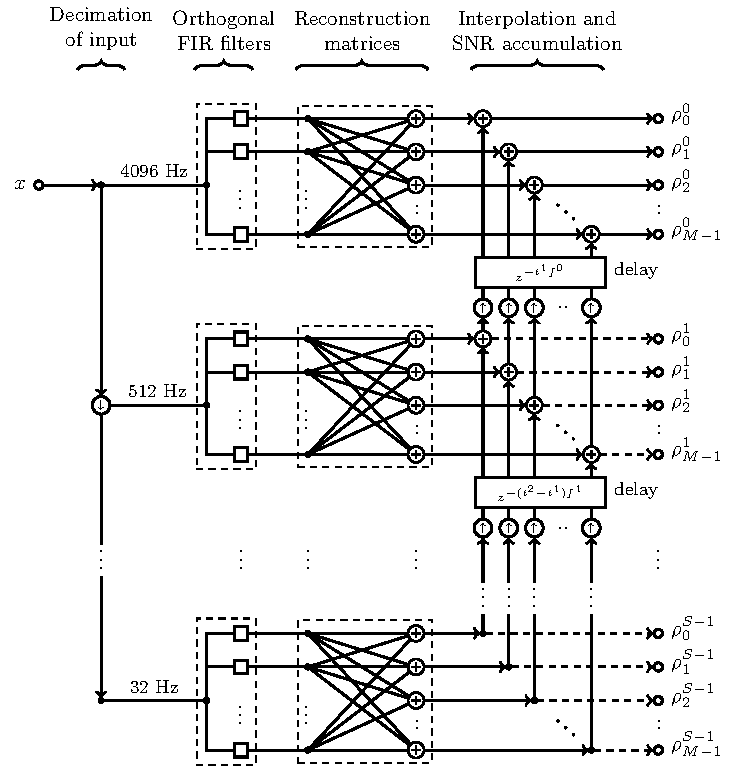
\includegraphics{figures/lloid-diagram.pdf}
	\caption{\label{fig:pipeline} Schematic of LLOID pipeline illustrating
signal flow.  Circles with arrows represent interpolation
\protect
\includegraphics{figures/upsample-symbol.pdf} or decimation
\protect
\includegraphics{figures/downsample-symbol.pdf}.  Circles with plus
signs represent summing junctions
\protect
\includegraphics{figures/adder-symbol.pdf}.  Squares
\protect
\includegraphics{figures/fir-symbol.pdf} stand for FIR filters.  Sample
rate decreases from the top of the diagram to the bottom.  In this diagram each
time slice contains three \fir\ filters that are linearly combined to produce
four output channels.  In a typical pipeline the number of \fir\ filters is
much less than the number of output channels.}
\end{figure}
%
%
The signal flow diagram drawn in figure \ref{fig:pipeline} contains several
distinct stages and parallel branches.  The stages are decimation, filtering
the data against the orthogonal templates, reconstruction of the original
template basis, interpolation and accumulation of the early warning and final
{\SNR}. 

In the next section we compute the expected computational cost scaling of this
decomposition and compare it with the brute-force time-domain implementation of
\eqref{eq:SNRTD} and higher latency frequency-domain methods.

\subsection{Comparison of computational costs}

We now examine the computational cost scaling of the approximate implementation
of a conventional time-domain or frequency-domain matched filter bank as compared
with \lloid{}.  For convenience, table~\ref{tab:recap} provides a review of the notation
that we will need in this section.
%
% symbols used in FLOPs calculations table
%
\Table{\label{tab:recap} Notation used to describe filters.}
\br
	& Definition \\
\mr
\numtmps		& number of templates \\
\tmpsamps	& number of samples per template \\
\numslices	& number of time slices \\
\numsvdtmps	& number of orthogonal templates in time slice $s$ \\
\slicessamps	& number of samples in time slice $s$ \\
$f^s$		& sample rate in time slice $s$ \\
$N^\shortdownarrow$ & number of coefficients in decimation filter \\
$N^\shortuparrow$ & number of coefficients in interpolation filter \\
\br
\end{tabular}
\end{indented}
\end{table}

\editorial{This section's two tables are small.  Any way to put them side by side or next to another figure?}

\Table{\label{table:flops}Minimum computational cost of the \fir{} filter bank, \fft{} convolution, and \lloid\ methods for a bank of 657 templates sampled at 4096 Hz.}
\br
Method & \flops \\
\mr
\fir{} & $2.4\times10^{13}$ \\
\fft{} convolution & $2.6\times10^8$ \\
\lloid & $4.7\times10^8$ \\
\br
\end{tabular}
\end{indented}
\end{table}

\subsubsection{Conventional time-domain method}

The conventional time-domain method consists of a bank of \fir{} filters, or sliding-window dot products.  If there are $\numtmps$ templates, each $\tmpsamps$ samples in length, then each filter requires $M N$ multiplications and additions per sample, or $2 \numtmps \tmpsamps f^0$ floating point operations per second (\flops) at a sample rate $f^0$.

\subsubsection{Conventional frequency-domain method}

The most common frequency-domain method is known as the \emph{overlap-save} algorithm, described in \cite{numerical-recipes-chapter-13}.  It entails splitting the input into blocks of $D$ samples, $D > \tmpsamps$, each block overlapping the previous one by $D - \tmpsamps$ samples.  For each block, the algorithm computes the forward \fft\ of the data and the templates, multiplies them, and then computes the reverse \fft.

Modern implementations of the \fft, such as the ubiquitous \texttt{fftw}, require about $2 \fftblock \lg \fftblock$ operations to evaluate a real transform of size $\fftblock$~\cite{Johnson:2007p9654}.  Including the forward transform of the data and $M$ reverse transforms for all of the templates, the \fft\ costs $2 (\numtmps + 1) \fftblock \lg \fftblock$ operations per block.  The multiplication of the transforms adds a further $2 \numtmps \fftblock$ operations per block.  Since each block produces $\fftblock - \tmpsamps$ usable samples of output, the overlap-save method requires
$$
f^0 \cdot \frac{2 (\numtmps + 1) \lg \fftblock + 2 \numtmps}{1 - \tmpsamps/\fftblock} \; \mathrm{\flops}.
$$

\subsubsection{\lloid\ method}

For time slices $s$, the \lloid\ method requires $2 \slicessamps \numsvdtmps f^s$ \flops\ 
for evaluating the orthogonal filters, $2 \numtmps \numsvdtmps f^s$ \flops\ for the 
linear transformation from the $\numsvdtmps$ basis templates to the $\numtmps$ time-sliced templates, and $\numtmps f^s$ \flops\ to add the resultant partial \SNR\ stream.

The computational cost of the decimation of the detector data is a little bit more subtle.  Decimation is achieved by applying an \fir\ antialiasing filter and then downsampling, or deleting samples in order to reduce the sample rate from $f^{s-1}$ to $f^s$.  Naively, an antialiasing filter with $N^\shortdownarrow$ coefficients should demand $2 N^\shortdownarrow f^{s-1}$ \flops.  However, it is necessary to evaluate the antialiasing filter only for the fraction $f^s / f^{s-1}$ of the samples that will not be deleted.  Consequently, an efficient decimator that requires only $2 N^\shortdownarrow f^{s-1} \cdot \left( f^s / f^{s-1} \right) = 2 N^\shortdownarrow f^s$ \flops\ is possible.

The story is similar for the interpolation filters used to change the sample rates of the partial \SNR{} streams.  Interpolation of a data stream from a sample rate $f^s$ to $f^{s-1}$ consists of inserting zeros between the samples of the original stream, and then applying a low-pass filter with $N^\shortdownarrow$ coefficients.  The low-pass filter requires $2 M N^\shortdownarrow f^{s-1}$ \flops.  However, by taking advantage of the fact that by construction a fraction $f^{s-1}/f$ of the samples are zero, it is possible to build an efficient interpolator that requires only $M N^\shortuparrow f^{s-1} \cdot \left( f^s / f^{s-1} \right) = 2 M N^\shortuparrow f^s$ \flops.

Taking into account the decimation of the detector data, the orthogonal \fir\ filters, the reconstruction of the time sliced templates, the interpolation of \SNR\ from previous time slices, and the accumulation of \SNR, in total \lloid\ requires
$$
\sum_{\mathclap{s=0}}^{\mathclap{S-1}} \left( 2 \slicessamps \numsvdtmps + 2 \numtmps \numsvdtmps + \numtmps \right) f^s + 2\sum_{\mathclap{f \in \{f^s\}}} \left( N^\shortdownarrow + \numtmps N^\shortuparrow \right) f \textrm{ \flops.}
$$
The second sum is carried out over the set of sample rates of all of the time slices rather than over the time slices themselves because some time slices may have the same sample rates.

\subsubsection{Extrapolation of the computational cost of the \lloid\ method to an Advanced LIGO search}

Table \ref{table:flops} shows that it requires about 0.5 GFLOPS to conduct the
filtering, reconstruction and resampling stages of the \lloid\ method for 657
templates chosen around typical NS--NS mass parameters.  Given the capability
of modern CPUs it should be possible to filter that sub-bank on one CPU.
Assuming that the cost holds for the other sub-banks we expect that the full
parameter space should require $\sim 150$ CPUs for realtime filtering with the
\lloid\ method per detector.  Even if real implementations fall short of these
estimates by factors of several, there will still be ample computing resources
for an early warning search in the advanced detector era.

\begin{comment}

% Do we want to spend this much copy on the whitener?
% What matters is that we have picked a low-latency whitening procedure.

\subsection{Data Whitening}
Matched filtering the SVD basis vectors has motivated a decoupling of the
whitening routine from the matched filtering engine. This was necessary in
order weight templates appropriately by whitening them before the SVD
calculation, and, as such, we have also moved the data whitening outside the
match filter engine. We have chosen to whiten the data using a running
geometric average of the PSD computed by Hann windowing 8 second buffers of
data and using 50\% overlapping buffers. The running geometric average is
updated once per buffer from a median of the recent PSDs. We find that this
algorithm is extremely fast to converge to an accurate PSD and also very robust
against glitches.

An inspiral, to leading order, has gravitational-wave frequency evolution given
by
%
\begin{equation}
%
f(t) = \frac{1}{8 \pi \mathcal{M}} \left( \frac{t_c - t}{5 \mathcal{M}}
\right)^{-3/8}\;,
%
\end{equation}
%
whose time derivative is given by
%
\begin{equation}
%
\frac{df}{dt} = \frac{3}{320 \pi \mathcal{M}^2} \left( \frac{t_c - t}{5
\mathcal{M}} \right)^{-11/8}\;.
%
\end{equation}
%
Combining these, we find the frequency evolution as a function of frequency to
be
%
\begin{equation}
%
\frac{df}{dt}(f_0) = \frac{3}{320 \pi \mathcal{M}^2} \left( 8 \pi \mathcal{M}
f_0 \right)^{3/11}\;,
%
\end{equation}
%
which can be inverted to get the minimum frequency which has a given frequency
derivative,
%
\begin{equation}
%
f_0 = \frac{1}{8 \pi \mathcal{M}} \left( \frac{320 \pi \mathcal{M}^2}{3}
\frac{df}{dt} \right)^{11/3}\;.
%
\end{equation}

If we allow frequency bins to be affected by an injection only once within the
median history, we need to calculate the corresponding $df/dt$ for our PSD
calculation. An FFT of a buffer with length $T$ will have a frequency
resolution $df = 1/(2T)$. Hann windowing the data and overlapping buffers by
50\% introduces correlations in neighboring frequency bins of the FFT. This
means that we actually want the frequency to change by $df = 3/(2T)$ before the
next PSD calculation, which happens a $dt = T/2$ later, resulting in a minimum
$df/dt = 3/T^2$.

Combining these results we find the lower frequency bound for our injections,
assuming a chirp mass for a binary with $m_1 = m_2 = 1 M_{\odot}$ and $T = 8$
s, is 23 Hz.

We want to compute the equivalent injection density which would be biased as
much as lalapps\_inspiral's PSD estimator, which allows $\sim3$ injections per
2048 seconds. It computes the PSD by breaking the segment up into 16 256 second
chunks. These chunks are then combined into to sets of 8 chunks each. The
median of each set is then averaged across the sets for each frequency bin to
produce the PSD estimate for that 2048 second segment. This procedure results
in an average injection density of 1.5 per 8 PSDs in the median history, which
is comparable to LLOID's 1 per 7 PSDs in the median history. Since LLOID has an
injection history of 7 PSDs which span 32 seconds, this means LLOID can perform
one injection every 32 seconds, or 64 injections per 2048 second segment, more
than an order of magnitude increase in density over lalapps\_inspiral.
\end{comment}


\section{Implementation}
\label{sec:implementation}

In this section we describe an implementation of the \lloid\ method described
in section \ref{sec:method} suitable for rapid gravitational-wave
searches for compact binary coalescence.  The \lloid\ method requires several
computations that can be completed before the analysis is underway.  Thus
we divide the procedure into two stages 1) an off-line planning stage and 2) an
online, low-latency filtering stage.  The off-line stage can be done before the
analysis is started and updated asynchronously, whereas the online stage must
keep up with the detector output and produce search results as rapidly as
possible.  In the next two subsections we describe what these stages entail.

\subsection{Planning stage}

The choice of filter waveforms and singular value decomposition can be done in
advance and will be valid as long as the detector noise spectrum remains
roughly constant.  New filter waveforms can be computed asynchronously using
updated spectrum estimates as they are available. 

\begin{figure}[htbp]
	\label{fig:tmpltbank}
	\begin{center}
		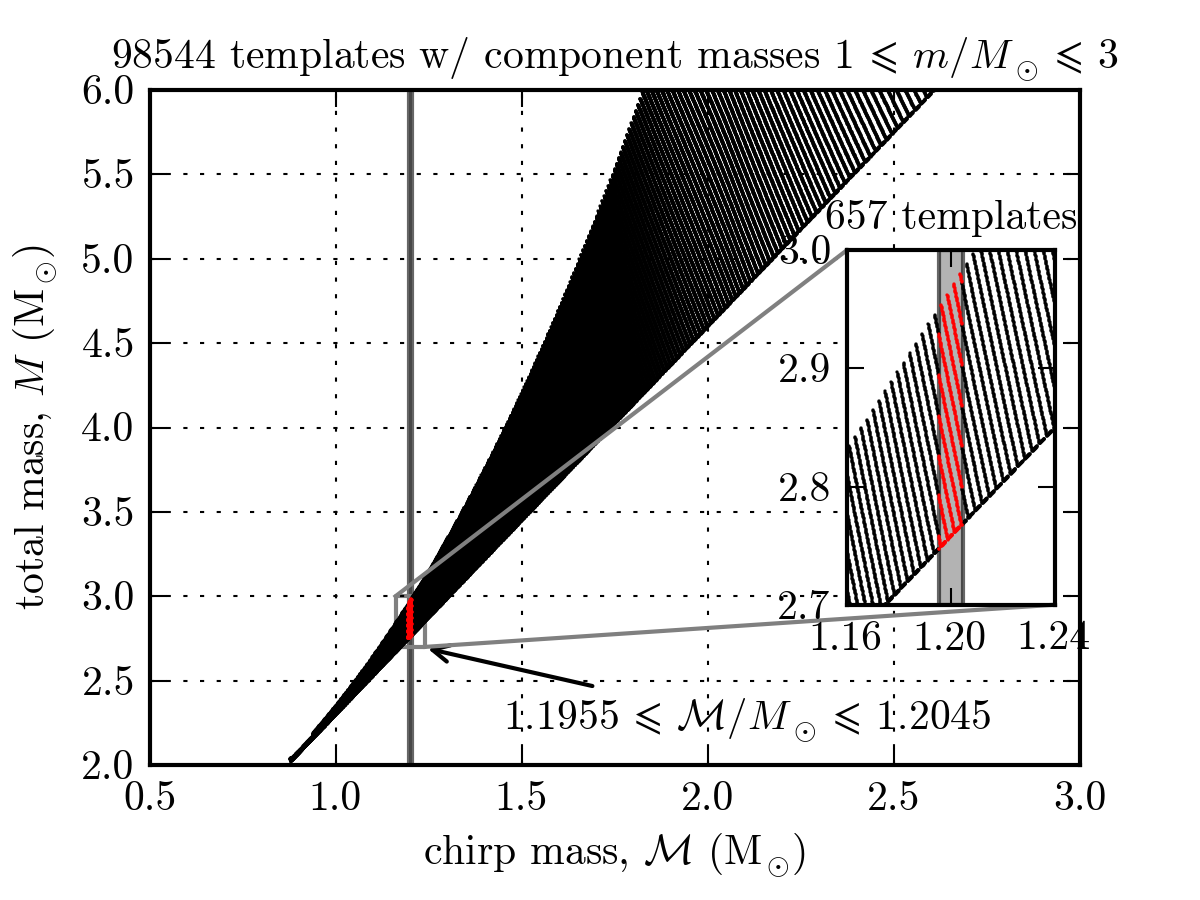
\includegraphics[scale=0.75]{figures/tmpltbank.png}
		\caption{Placement of template parameters used in this paper.  The template bank consists of 98544 templates with component masses $m_1$, $m_2$, between 1~and~3~$M_\odot$.  We shall design a filter bank to search for a small subset of these template parameters with chirp masses $\mathcal M$ between 1.1955~and~1.2045~$M_\odot$.}
	\end{center}
\end{figure}

\begin{table}
\begin{indented}
\caption{Filter design for these 657 templates.  From left to right, this table shows the sample rate, time interval, number of samples, and number of orthogonal templates for each time slice.  The \textsc{svd} tolerance is varied from $\left(1-10^{-1}\right)$ to $\left(1-10^{-6}\right)$}
\item[]\begin{tabular}{rr@{,}lc*{6}{r}}
\br
\multicolumn{4}{c}{} &\centre{6}{$\log_{10}$ (1 - \textsc{svd} tolerance)} \\
\ns
\multicolumn{4}{c}{} &\crule{6} \\
$f^s$ (Hz) & $(t^{s+1}$&$t^s]$ (s) & $N^s$ & -1 & -2 & -3 & -4 & -5 & -6 \\
\mr
4096 & (0.5&0] & 2048 & 1 & 4 & 6 & 8 & 10 & 14 \\
512 & (4.5&0.5] & 2048 & 2 & 6 & 8 & 10 & 12 & 16 \\
256 & (12.5&4.5] & 2048 & 2 & 6 & 8 & 10 & 12 & 15 \\
128 & (76.5&12.5] & 8192 & 6 & 20 & 25 & 28 & 30 & 32 \\
64 & (140.5&76.5] & 4096 & 1 & 8 & 15 & 18 & 20 & 22 \\
64 & (268.5&140.5] & 8192 & 1 & 7 & 21 & 25 & 28 & 30 \\
64 & (396.5&268.5] & 8192 & 1 & 1 & 15 & 20 & 23 & 25 \\
32 & (460.5&396.5] & 2048 & 1 & 1 & 3 & 9 & 12 & 14 \\
32 & (588.5&460.5] & 4096 & 1 & 1 & 7 & 16 & 18 & 21 \\
32 & (844.5&588.5] & 8192 & 1 & 1 & 8 & 26 & 30 & 33 \\
32 & (1100.5&844.5] & 8192 & 1 & 1 & 1 & 12 & 20 & 23 \\
\end{tabular}
\end{indented}
\end{table}

The planning stage begins with choosing templates that cover the space of mass
parameters with a hexagonal grid~\cite{PhysRevD.76.102004} in order to satisfy
a minimum match criterion.  This assures a user-specified, maximum loss in \SNR\
for signals that fall in-between the chosen templates.  Typically the minimum
match is 97\% corresponding to a maximum mismatch of 3\%.  Next, the templates
are subdivided into groups of neighbors called ``sub-banks'' that are
appropriately sized so that each bank can be efficiently handled by a single
computer.  The neighbors are chosen to have comparable chirp mass, which produces
sub-banks with very similar waveforms.  Dividing the mass space into smaller
sub-banks reduces the computational cost of the singular value decomposition
and is the approach considered in~\cite{Cannon:2010p10398}.  Using our
understanding of the time-frequency evolution of the templates, we choose time
slice boundaries as in \eqref{FIXME} such that all of the templates within a
sub-bank are sub-critically sampled at progressively lower sample rates.  Next,
the templates within the sub-bank are realized as \fir\ filter
coefficients.  For each time slice, the templates are down-sampled to the
appropriate sample rate.  Finally, the \SVD\ is applied to each time
slice in the sub-bank in order to produce a set of orthogonal \fir\
filters and a reconstruction matrix that maps them back to the original
templates as described in \eqref{FIXME}.  The down-sampled orthogonal
\fir\ filter coefficients, the reconstruction matrix, and the time slice
boundaries are all saved to disk.

\subsection{Filtering stage}

The \lloid\ algorithm could be used in a true sample-in-sample-out real-time
system.  However, such a system would likely require integration directly into
the data acquisition and storage system of the gravitational wave
observatories.  A slightly more modest goal is to leverage existing low
latency, but not real-time, signal processing infrastructure in order to
implement the \lloid\ algorithm.  For the near-term this should be a viable 
solution for ultra-low latency searches with $\sim 1s$ intrinsic latency.

We have implemented a prototype of the low latency filtering stage using an
open source signal processing environment called \gstreamer\ \cite{gstreamer}.
\gstreamer\ is a vital component of many Linux systems, providing media
playback, authoring, and streaming on devices from cell phones to desktop
computers to streaming media servers.  Given the similarities of gravitational
wave detector data to audio data it is not surprising that \gstreamer\ is
useful for our purpose. \gstreamer\ also provides some useful stock signal
processing elements such as resamplers and filters.  We have extended the
\gstreamer\ framework by developing custom elements that are available in the
\gstlal\ library~\cite{gstlal}.  Figure \ref{fig:pipeline} describes
schematically how we implement the \lloid\ algorithm using \gstlal\ and
\gstreamer\ components.
%
%
\begin{figure}[htbp]
	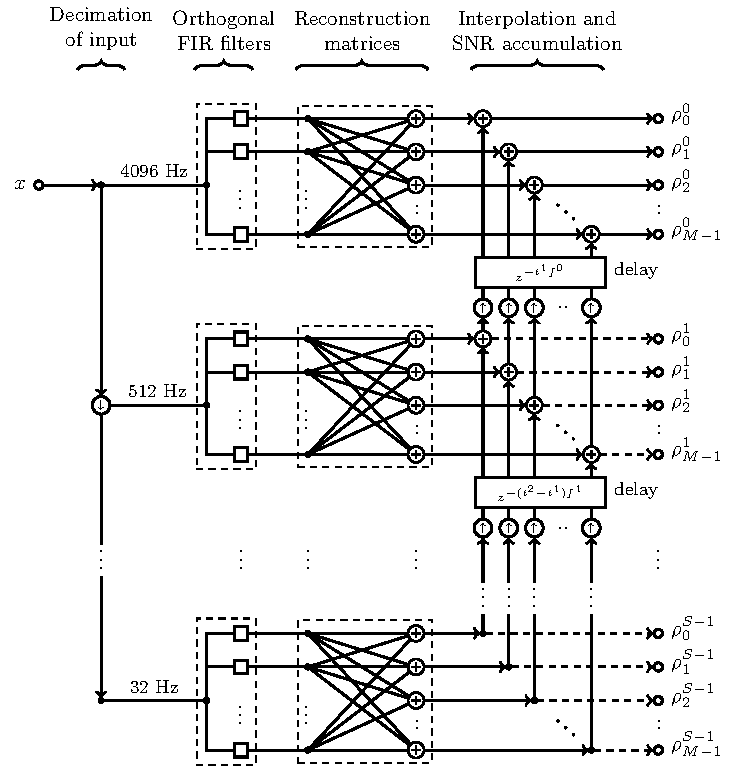
\includegraphics{figures/lloid-diagram.pdf}
	\caption{\label{fig:pipeline} Schematic of LLOID pipeline illustrating
signal flow.  Circles with arrows represent up-sampling
\protect
\includegraphics{figures/upsample-symbol.pdf} or down-sampling
\protect
\includegraphics{figures/downsample-symbol.pdf}.  Circles with plus
signs represent summing junctions
\protect
\includegraphics{figures/adder-symbol.pdf}.  Squares
\protect
\includegraphics{figures/fir-symbol.pdf} stand for FIR filters.  Sample
rate decreases from the top of the diagram to the bottom.  In this diagram each
time slice contains three \fir\ filters that are linearly combined to produce
four output channels.  In a typical pipeline the number of \fir\ filters is
much less than the number of output channels.}
\end{figure}

The filter pipeline drawn in figure \ref{fig:pipeline} consists of several
distinct stages and parallel branches.  The stages are decimation, filtering
the \SVD\ basis, reconstruction of the original template basis, interpolation
and accumulation of the early warning and final {\SNR}.  We outline the stages
below. 

\subsubsection{Decimation}

First, the sample rate of the whitened detector data is reduced to successively
lower sample rates by decimation.  Decimation involves applying an anti-aliasing
filter to the data, and then down-sampling by deleting samples.  We use a
192-tap \fir\ decimator provided by {\tt Gstreamer's audioresample}
element.  The detector data is provided at every power-of-two sample rate
required by the template time slices described in \eqref{eq:time-slices}.  These
parallel decimated data streams are fed into parallel fir filter banks in the
next stage.

\subsubsection{Orthogonal \fir\ filters}

The \fir\ filter banks are implemented using a \gstlal\ element called {\tt
lal\_firbank}, which produces N channels of filter output from an NxM matrix of
\fir\ filter coefficients.  This element is used in parallel branches in the
pipeline to implement the filtering of the \SVD\ basis filters in each time
slice.  Rather than implement the time sliced templates as zero padded \fir\
filters as described in \eqref{eq:time-slices} we instead implement them as shorter
filters that contain only the nonzero samples.  Adding the appropriate time
offset to the filter output later in the pipeline makes up for the lack of
explicit zero padding.  The orthogonal filter outputs must be reconstructed
into the filter output for the underlying physical filter outputs. 

\subsubsection{Reconstruction}

The orthogonal filter output provided by the \SVD\ must be used in linear
combinations in order to obtain the physical filter output for the template
waveforms.  This involves a matrix multiplication.  We use a \gstlal\ element
called {\tt lal\_matrixmixer} on the output of each orthogonal filter bank in
order to produce the filter output for the original waveforms in each time
slice.  At this point the time slice filter outputs are not yet at the same
sample rate, however, before they are up-sampled we sum the reconstructed output
of any time slices that have a common sample rate.

\subsubsection{Interpolation}

Before we can construct the final \SNR\, the individual time slice filter
outputs must be brought to a common sample rate, or up-sampled.  This is done
using the same \gstreamer\ element as was used for decimation, {\tt
audioresample}.  

\subsubsection{\SNR\ accumulation}

In order to accumulate \SNR\ for an early warning, the time slice filter
output is up-sampled to the next highest frequency time slice and summed. This
process is iterated until the final \SNR\ is computed.  However at each stage
of up-sampling the summed filter outputs are related to the early warning \SNR\
by a simple normalization factor that can be computed in advance. Thus the
\lloid\ algorithm and this implementation leads to a simple early warning
pipeline with little additional work.


\section{Results}
\label{sec:results}

In this section we evaluate the accuracy of the \lloid{} algorithm using our 
\gstreamer{}-based implementation described in the previous section. We calculate the
measured \SNR\ loss due to the approximations of the \lloid\ method and our
implementation of it. Using a configuration that gives acceptable \SNR{} loss for
our chosen set of source parameters, we then compare the computational cost in \flops\
for \TD\ method, the \FD\ method, and \lloid.

\subsection{Setup}
\label{sec:bank-setup}

We examine the performance of the \lloid\ algorithm on a small region of
compact binary parameter space centered on typical \textsc{ns}--\textsc{ns}
masses.  We begin by constructing a template bank that spans component masses
between 1~and~3~$M_\odot$ using a simulated Advanced \LIGO{} noise
curve~\citep{ALIGONoise}.  This results in a grid of 98544 points, or
$2 \times 98544 = 197088$~templates.  Then we create sub-banks by partitioning
the parameter space by chirp mass.  We shall concentrate on a sub-bank with 657
chirp masses between 1.1955 and 1.2045~$M_\odot$, or $2 \times 657 = 1314$~templates.
Figure \ref{fig:tmpltbank} illustrates this procedure.
\begin{figure}[h]
	\plotone{figures/tmpltbank.pdf}
	\caption{\label{fig:tmpltbank}Source parameters selected for sub-bank used in this
case study, consisting of component masses $m_1$, $m_2$, between 1 and 3~$M_\odot$, and
chirp masses $\mathcal{M}$ between 1.1955 and 1.2045~$M_\odot$.}
\end{figure}
With this sub-bank we were able to construct an efficient time-slice decomposition
that consisted of 11 time slices with sample rates between 32 and 4096 Hz summarized
in Table~\ref{tab:time_slices}.
\begin{table*}
\caption{\label{tab:time_slices} Filter design sub-bank of 657 templates.  From left to right, this table shows the sample rate, time interval, number of samples, and number of orthogonal templates for each time slice.  We vary \SVD{} tolerance from $\left(1-10^{-1}\right)$ to $\left(1-10^{-6}\right)$.}
\begin{center}
\begin{minipage}[c]{0.4\textwidth}
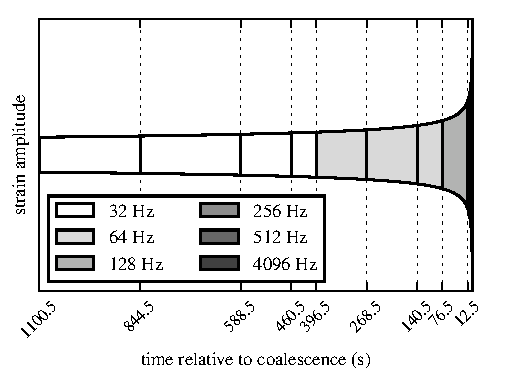
\includegraphics{figures/envelope}
\end{minipage}
\begin{minipage}[c]{0.55\textwidth}
\begin{tabular}{rr@{,\,}lc*{6}{r}}
\tableline\tableline
\\ [-2ex]
$f^s$ & $[t^s$&$t^{s+1})$ & &\multicolumn{6}{c}{$-\log_{10}$ (1$-$\SVD{} tolerance)} \\% [1ex]
\cline{5-10}
\\[-2.5ex]
(Hz) & \multicolumn{2}{c}{(s)} & $N^s$ & $1$ & $2$ & $3$ & $4$ & $5$ & $6$ \\ \tableline
4096 & [0&0.5) & 2048 & 1 & 4 & 6 & 8 & 10 & 14 \\
512 & [0.5&4.5) & 2048 & 2 & 6 & 8 & 10 & 12 & 16 \\
256 & [4.5&12.5) & 2048 & 2 & 6 & 8 & 10 & 12 & 15 \\
128 & [12.5&76.5) & 8192 & 6 & 20 & 25 & 28 & 30 & 32 \\
64 & [76.5&140.5) & 4096 & 1 & 8 & 15 & 18 & 20 & 22 \\
64 & [140.5&268.5) & 8192 & 1 & 7 & 21 & 25 & 28 & 30 \\
64 & [268.5&396.5) & 8192 & 1 & 1 & 15 & 20 & 23 & 25 \\
32 & [396.5&460.5) & 2048 & 1 & 1 & 3 & 9 & 12 & 14 \\
32 & [460.5&588.5) & 4096 & 1 & 1 & 7 & 16 & 18 & 21 \\
32 & [588.5&844.5) & 8192 & 1 & 1 & 8 & 26 & 30 & 33 \\
32 & [844.5&1100.5) & 8192 & 1 & 1 & 1 & 12 & 20 & 23 \\
\tableline
\end{tabular}
\end{minipage}
\end{center}
\end{table*}
We use this sub-bank and decomposition for the remainder of this section.

\subsection{Measured \SNR\ loss}

The \SNR\ loss is to be compared with the mismatch of 0.03 that arises from the
discreteness of template bank designed for a minimal match of 0.97.  We will consider
an acceptable target \SNR\ loss to be a factor of 10 smaller than this, that is, no more
than 0.003.

We expect two main contributions to the \SNR\ loss to arise in our
implementation of the \lloid\ algorithm.  The first is the \SNR\ loss due to
the truncation of the \SVD\ at $L^s < M$ basis templates.  As remarked upon in
\citet{Cannon:2010p10398} and section~\ref{sec:svd}, this effect is measured by
the \SVD\ tolerance.  The second comes from the limited bandwidth of the
interpolation filters used to match the sample rates of the partial \SNR\ streams.
The maximum possible bandwidth is determined by the length of the filter,
$N^\shortuparrow$.  \SNR\ loss could also arise if the series rather than parallel
connection of the decimation and interpolation filters reduces their bandwidth
measurably, if the decimation and interpolation filters do not have perfectly uniform
phase response, or if there is an unintended subsample time delay at any stage.

To measure the accuracy of our \gstreamer\ implemention of \lloid\ including all of
the above potential sources of \SNR\ loss, we conducted impulse response tests.  The
\gstreamer\ pipeline was presented with an input consisting of a unit impulse.  By
recording the outputs, we can effectively ``play back'' the templates.  These impulse
responses will be similar, but not identical, to the original, nominal templates.  By
taking the inner product between the impulses responses for each output 
channel with the corresponding nominal template, we can gauge exactly how much \SNR\
is lost due to the approximations in the \lloid\ algorithm and any of the technical
imperfections mentioned above.  We call one minus this dot product the \emph{mismatch}
relative to the nominal template.

\paragraph{Effect of \SVD\ tolerance}

We studied how the \SVD\ tolerance affected \SNR\ loss by holding
$N^\shortuparrow = 192$ fixed as we vaired the \SVD\ tolerance from
$\left(1-10^{-1}\right)$ to $\left(1-10^{-6}\right)$.  The minimum, maximum, and median
mismatch are shown as functions of \SVD\ tolerance in
Figure~\ref{fig:bw}a.  As the \SVD\ tolerance increases toward 1, the
\SVD\ becomes an exact matrix factorization, but the computational cost increases as
the number of basis filters increases.  The conditions presented here are more
complicated than in the original work~\citep{Cannon:2010p10398} due to the inclusion
of the time-sliced templates and interpolation, though we still see that the average
mismatch is approximately proportional to the \SVD\ tolerance down to
$\left(1-10^{-4}\right)$.  However, as the \SVD\ tolerance becomes even higher, the
mismatch seems to saturate around $2 \times 10^{-4}$.  This could be the effect of the
interpolation, or an unintended technical imperfection that we did not model or expect.
However, this is still an order of magnitude below our target mismatch of 0.003.  We
find that an \SVD\ tolerance of $\left(1-10^{-4}\right)$ is adequate to achieve our
target \SNR{} loss.

\paragraph{Effect of interpolation filter length}

Next, keeping the \SVD\ tolerance fixed at $\left(1-10^{-6}\right)$, we studied the
impact of the length $N^\shortuparrow$ of the interpolation filter.  The mismatch as
a function of $N^\shortuparrow$ is shown in Figure~\ref{fig:bw}b.  The
mismatch saturates at $\sim$$2 \times 10^{-4}$ with $N^\shortuparrow = 64$.  We find
that a filter length of 16 is sufficient to meet our target mismatch of 0.003.

\begin{figure*}[b]
	\begin{minipage}[t]{0.5\textwidth}
		\begin{center}
			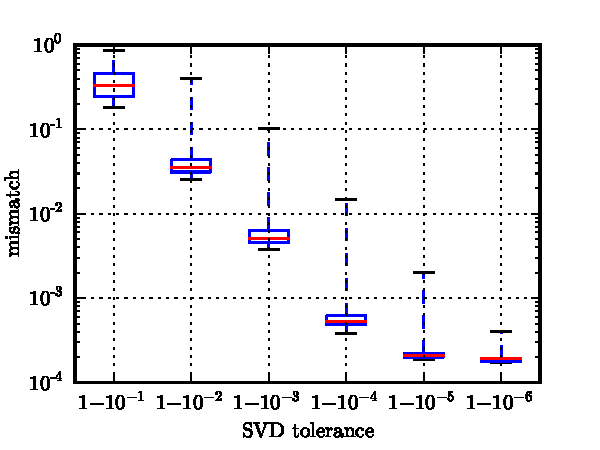
\includegraphics{figures/bw.pdf}
			(a) Mismatch versus \SVD\ tolerance
		\end{center}
	\end{minipage}
	\begin{minipage}[t]{0.5\textwidth}
		\begin{center}
			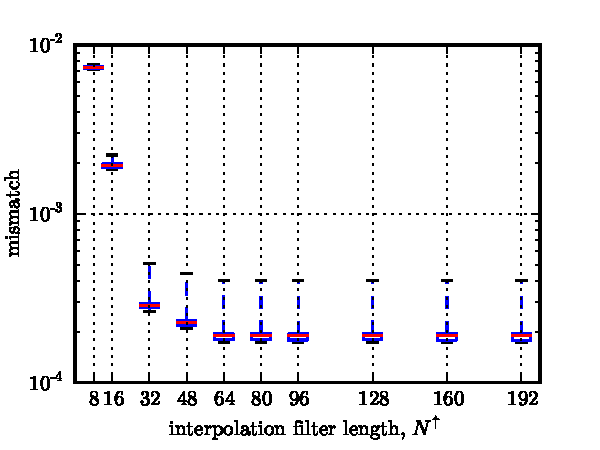
\includegraphics{figures/bw_resample.pdf}
			(b) Mismatch versus $N^\shortuparrow$
		\end{center}
	\end{minipage}
	\caption{\label{fig:bw}Box-and-whisker plot of mismatch between nominal
template bank and \lloid\ measured impulse responses.  The upper and lower boundaries of
the boxes show the upper and lower quartiles; the lines in the center denote the medians.
The whiskers represent the minimum and maximum mismatch over all templates.  In 
(a) the interpolation filter length is held fixed at $N^\shortuparrow = 192$, while
the \SVD\ tolerance is varied from $\left(1-10^{-1}\right)$ to $\left(1-10^{-6}\right)$.
In (b), the \SVD\ tolerance is fixed at $\left(1-10^{-6}\right)$ while $N^\shortuparrow$
is varied from 8 to 192 coefficients.}
\end{figure*}

\subsection{Lower bounds on computational cost and latency compared to other
methods}

We are now prepared to offer the estimated computational cost of filtering this
sub-bank of templates compared to other methods.  We used the results of the
previous subsections to set the \SVD\ tolerance at $\left(1-10^{-4}\right)$ and
the interpolation filter length to 16. Table~\ref{table:flops} shows the
computational cost in \flops\ for this sub-bank.  For the \FD\ method, an \fft\
block size of $\fftblock = 2 \tmpsamps$ is assumed, resulting in a latency of
$\left(\tmpsamps f^0\right)$ seconds.  Both the \FD\ method and \lloid\ are
five orders of magnitude faster than the conventional \TD\ method.  However,
the \FD\ method has a latency of over half of an hour, whereas \lloid\ has no
latency at all.
%
\begin{table}
\caption{\label{table:flops}Computational cost in \flops\ of the \TD\ method, the \FD\ method, and \lloid\ for the sub-bank described in section~\ref{sec:bank-setup}.}
\begin{center}
\begin{tabular}{lll}
\tableline\tableline
method & \flops\ & latency (s) \\
\tableline
time domain & $2.4\times10^{13}$ & 0 \\
frequency domain & $2.6\times10^8$ & $2\times10^3$ \\
\lloid\ (theory) & $4.7\times10^8$ & $2\times10^{-3}$ \\
\lloid\ (prototype) & ----------- & 5 \\
\tableline
\end{tabular}
\end{center}
\end{table}

\subsection{Extrapolation of the computational cost to an Advanced \LIGO{} search}

Table~\ref{table:flops} shows that the \lloid\ method requires $\sim$$10^8$
\flops\ to cover a sub-bank comprising $\sim$$10^2$ out of the total $\sim$$10^5$
mass pairs.  Given that modern (ca. 2011) workstations can sustain computation
rates up to $\sim$$10^{10}$ \flops{}, and assuming that other regions of the
parameter space have similar computational scaling, an entire single detector
search could be implemented with $\gtrsim$$10$ machines.  Template length does
vary over the parameter space; lower-mass templates are longer and would
require more computation to analyze while higher-mass templates are shorter and
would require less. However, we consider the estimates based on this sub-bank
to be a reasonable representation.

By comparison, using the \TD\ method to achieve the same latency costs
$\sim$$10^{13}$ \flops\ for this particular sub-bank, and so it would require
$\sim$$10^6$ present-day machines to search the full parameter space.
Presently, the \LIGO{} Data Grid consists of only $\sim$$10^4$ machines.

\subsection{Measured latency and overhead}

Our \gstreamer\ pipeline for measuring impulse responses contained
instrumentation that would not be necessary for an actual search, including
additional interpolation filters to bring the early-warning outputs back to the
full sample rate and additional outputs for recording signals to disk.

We wrote a second, stripped pipeline to evaluate the actual latency and
computational overhead.  We executed this pipeline on one of the submit
machines of the \LIGO-Caltech cluster, a Sun Microsystems Sun
Fire\texttrademark\ X4600~M2 server with eight quad-core 2.7~GHz AMD
Opteron\texttrademark\ 8384 processors.  This test consumed 78\% of the
capacity of just one out of the 32 cores, maintaining a constant latency of
5~s.

The measured overhead is consistent to within an order of magnitude with the
lower bound from the \flops\ budget.  The additional overhead is probably
dominated by thread synchronization.  A carefully optimized \gstreamer\
pipeline or a hand-tuned C implementation of the pipeline might reduce overhead
further.

The 5~s latency is probably due to buffering and synchronization.  The latency
might be reduced by carefully tuning buffer lengths at every stage in
the pipeline.  The minimum theoretically possible latency is set by
$N^\shortdownarrow$ and $N^\shortuparrow$.

Even without further refinements, our implementation of the \lloid\ algorithm
achieves latencies that would make other aspects of the analysis the limiting
steps assuming that the human vetting process is automated.  


\section{Conclusions}
\label{SECV}\label{sec:conclusions}

We have demonstrated a computationally feasible procedure for the rapid and
even preemptive detection of \GW{}s emitted during the coalescence
of neutron stars and stellar-mass black holes. Our method is as fast as
standard \fft{} convolutions but allows for zero latency, sample-in-sample-out
operation.  Our search targets are expected to produce prompt electromagnetic
signals and may be the progenitors of some short hard gamma-ray bursts.  Rapid
alerts to the broader astronomical community will improve the chances of
detecting an electromagnetic counterpart in bands from gamma-rays down to
radio.  We anticipate requiring $\sim100$ modern multi-core computers to
analyze a four-detector network of \GW{} data for binary neutron
stars and stellar-mass black holes.  This is well within the current computing
capabilities of the \LIGO{} Data Grid~\cite{LDG}. In the future, this could be
improved upon further by conditionally reconstructing the \SNR{} time-series
only during times when a composite dection statistic crosses a
threshold~\cite{svd-compdetstat}.

The algorithm we described has no intrinsic latency.  However, there are
fundamental and practical latencies associated with the analysis and detection
procedure. For example, the \LIGO{} detectors, data acquisition is synchronized
to a 1/(16~Hz) cadence, introducing an up-front latency~\cite{CITE_CDS}. Data
aggregation from
the observatories will travel over various networks, each capable of high
bandwith but perhaps only modest latency.  This could amount to a similar
latency of $\sim$100 ms.  Lastly, unless a real-time infrastructure is adopted
post data acquisition, it is likely that there will be an inherent latency
introduced by such infrastructure.  We have shown a prototype implementation
of \lloid{} using \gstlal\ that is capable of order seconds latency. Based
on our experience, significant work would have to be done in order to improve
upon this number, for example, more tightly integrating analysis and data
acquisition. This should be considered for third-generation detector design.

Although we have demonstrated a feasible method for advance detection we have
not explored the accuracy of sky localization that is possible before merger.
Ref.~\cite{Fairhurst2009} discusses some of the theoretical prospects for early sky
localization.  Our future work will explore the prospects of early-warning
detection with realistic simulations of binary mergers using the infrastructure
and techniques described here. 

\editorial{nvf: It's a bit pie-in-the-sky, but we could also mention reconfiguring
the signal recycling mirror to optimize SNR at merger. There's a lot of science there.}

%Latency budget, including `before' and `after' quotes for:

%\begin{itemize}
%\item Data acquisition
%\item Calibration
%\item Data aggregation
%\item Analysis
%\item Localization
%\item Alert
%\item Telescope actuation
%\item Total
%\end{itemize}

%Future work:

%\begin{itemize}
%\item Sub-solar mass search
%\item Hierarchical detection
%\end{itemize}


\acknowledgments
\textsc{ligo} was constructed by the California Institute of Technology
and Massachusetts Institute of Technology with funding from the National
Science Foundation and operates under cooperative agreement
\textsc{phy}-\oldstylenums{0107417}. This paper has \textsc{ligo} Document
Number \textsc{ligo}-\textsc{p}\oldstylenums{0900004}-v\oldstylenums{1}.

\appendix
\section{Filter bank for generating mock Advanced {\sc ligo} strain data}
\label{appendix:mock-data}

The filter bank described below reproduces the ``zero detuning, high power'' Advanced \textsc{ligo} noise model of  \cite{Shoemaker:2009p9770} very faithfully.  Since it is composed of a small number of third order or lower linear filters, a digital implementation of it can produce mock data in realtime with negligibly few floating point operations.

First, generate 5 independent streams of white Gaussian noise, $x_1, \dots, x_5$, sampled at 16384 Hz.  Next, the apply the (\textsc{f}/\textsc{i})\textsc{ir} filters described in equation~(\ref{eq:iirbank}) to generate $y_1, \dots, y_5$ from $x_1, \dots, x_5$ respectively.  Finally, sum and scale all of the $y_1, \dots, y_5$ together to obtain the final output $y$.

The power spectrum of $y$ is the sum of squares of the magnitudes of the transfer functions of all of the filters.  The output of the filter bank is compared with the noise model in Figure~\ref{fig:mock-psd} below.

The mock Advanced \textsc{ligo} noise generator is implemented by the GStreamer element \texttt{lal\_fakeadvligosrc}, which is included with the analysis code.

\begin{eqnarray}
\label{eq:iirbank}
\fl x_i &[n] \sim& \mathcal{N}[0, 1] \quad \forall \, i, n \nonumber\\\noalign{\vskip 2mm}
\fl y_1 &[n] =& \left(4 \times 10^{-28}\right) x_1[n] - y_1[n-1] + 2 \cdot .99995 \cos \left(\frac{2\pi \cdot 9.103}{16384}\right) y_1[n-2] - .99995^2 y_1[n-3] \nonumber\\\noalign{\vskip 2mm}
\fl y_2 &[n] =& \left(1.1 \times 10^{-23}\right) (x_2[n] - x_2[n-1]) \nonumber\\\noalign{\vskip 2mm}
\fl y_3 &[n] =& \left(10^{-27}\right) x_3[n] - y_3[n-1] + 2 \cdot .999 y_3[n-2] - .999^2 y_3[n-3] \nonumber\\\noalign{\vskip 2mm}
\fl y_4 &[n] =& \left(4 \times 10^{-26}\right) x_4[n] - y_4[n-1] + 2 \cdot .87 \cos \left(\frac{2\pi \cdot 50}{16384}\right) y_4[n-2] - .87 ^ 2 y_4[n-3] \nonumber\\\noalign{\vskip 2mm}
\fl y_5 &[n] =& \left(6.5 \times 10^{-24}\right) x_5[n] - y_5[n-1] - 2 \cdot .45 y_5[n-2] - .45 ^ 2 y_5[n-3] \nonumber\\\noalign{\vskip 2mm}
\fl \; y &[n] =& \frac{3\sqrt{16384}}{4} \left(y_1[n] + y_2[n] + y_3[n] + y_4[n] + y_5[n]\right)
\end{eqnarray}

\begin{figure}[h!]
\begin{center}
\includegraphics[scale=0.4]{mock_psd.pdf}
\caption{Power spectrum of 100 s of output from mock data filter bank compared with the ``zero detuning, high power'' Advanced \textsc{ligo} noise model.}
\label{fig:mock-psd}
\end{center}
\end{figure}

Note that the \textsc{cpu} overhead of this procedure will be entirely dominated by drawing the pseudorandom numbers $x_1, \dots, x_5$.


\section{Floating point operation counts}

\editorial{I just yanked this from the methods section.  It needs to be made more concise, maybe turned into a table of CPU budgets for various components of LLOID.} The filter bank can be implemented using finite impulse response (\textsc{fir}) filters, which are just sliding window dot products.  If there are $M$ templates of length $n$, and the data stream contains $N$ samples, then applying the filter bank requires $2 M N n$ operations.

More commonly, the matched filters are implemented using the \textsc{fft} convolution.  This entails applying \textsc{fft}s to blocks of $D$ samples, with $2 n \leq D$, each block overlapping the previous one by $n$ samples.  There are $N/(D-n)$ such blocks.  Modern implementations of the Cooley-Tukey \textsc{fft}, such as the ubiquitous \texttt{fftw}, require about $4 N \lg N$ operations to evaluate a \textsc{dft} of size $N$~\cite{Johnson:2007p9654}.  \editorial{This is more commonly known as ``overlap-save''.  We should find someone else's operation count and cite it.}  A $D$ sample cross-correlation consists of a forward \textsc{fft}, an $D$ sample dot product, and an inverse \textsc{fft}, totaling $8 D \lg N + 2 D$ operations per block.  Per sample, this is $(8 \lg D + 2) / (1 - n/D)$ operations. \editorial{Drew: Why don't we change this to an overlap of $m$ samples so we can see what happens as we increase the overlap to reduce latency.}

The \textsc{fir} filter implementation has the advantage that it has no intrinsic latency, whereas the \textsc{fft} convolution has at least the latency of the \textsc{fft} block size $D \geq 2 n$.  \editorial{Drew: Should the latency be D-n?} For example, for a $1.4 - 1.4 \, M_\odot$ template with duration $\sim 1 \, \mathrm{ks}$, the \textsc{fft} convolution has a latency $\geq 2 \, \mathrm{ks}$.  However, the \textsc{fir} filter implementation has the disadvantage of much greater overhead per sample than the \textsc{fft} convolution.  For a $1\,\mathrm{ks}$ template sampled at $4096\,\mathrm{Hz}$, the \textsc{fir} implementation requires about about $n / 8 \lg 2 n = 2.2 \times 10^4$ times more operations per sample than the \textsc{fft} implementation.



\begin{comment}
% Let's make glitch rejection in LLOID a separate paper.

\section{better noise model}

The assumption that the interferometer noise is well-modeled by a multivariate normal distribution is convenient, but false.  The presence of `glitches' in the interferometer, where the noise statistics change dramatically, is well documented.  Current methods, including ours in the form proposed in the paper, are easily fooled by these bursts of excess power, simply because the analyses assume that the only way that extra power can be introduced to the interferometer is by a gravitational wave.  The gravitational wave hypothesis $H_\mathrm{signal}$ will do a very poor job of explaining temporally coincident incoherent bursts of noise power in the interferometer, but the noise hypothesis $H_\mathrm{signal}$ in its simple form does even worse; the gravitational wave explanation is thus preferred.

We can generalize the noise hypothesis to cope with glitches by creating a model for glitches and adding that hypothesis to the set under consideration.  Like gravitational waves, glitches are infrequent, have poorly known waveforms, and poorly known power.  Unlike gravitational waves, they will not be correlated between instruments.

%The Gursel-Tinto method is not robust against interferometer glitches (nor does it claim to be; real interferometer data doesn't follow the normal distribution assumed in the derivation of the method.)  This is a problem in naive attempts to use the Gursel-Tinto algorithm as a search.  Excess energy of any almost any kind will be interpreted as a evidence of a gravitational wave.  An \emph{ad hoc} addition to the method was propsed in \cite{us}.  A better way forward is to use a noise model that more accurately reflects the 'bursty' or 'glitchy' nature of the data, by replacing the normal noise distribution with a long-tailed distribution.  An immediate problem is that the marginalization integral does not in general have a closed form solution for such distributions.  If we model the long-tailed distribution using two normal distributions the marginalization integral remains tractable.

One first attempt at such a hypothesis is to propose that an interferometer is either `quiet' with some probability $p(H_\mathrm{quiet}|H_\mathrm{noise})$ and has a unit normal noise distribution, or is `glitching' with probability $p(H_\mathrm{glitch}|H_\mathrm{noise})$ and has an increased standard deviation $\sigma_g$

\begin{equation}
P(\mathbf{x}|H_\mathrm{noise})
=
\prod_{i=1}^{N}\left[p(H_\mathrm{quiet}|H_\mathrm{noise})
(2\pi)^{-n/2}
\exp(-\frac{1}{2}\sum_{j=1}^n x_{ij}^2)
+p(H_\mathrm{glitch}|H_\mathrm{noise})
(2\pi)^{-n/2}\sigma_g^{-n}
\exp(-\frac{1}{2\sigma_g^2}\sum_{j=1}^n x_{ij}^2)
\right]\label{eq:glitchy}
\end{equation}

If there is excess energy in only one detector, the new noise hypothesis will readily explain it.  If there is excess energy in three detectors, the noise hypothesis must invoke three coincident glitches and is penalized by $p(H_\mathrm{glitch}|H_\mathrm{noise})^3$ reflecting our belief that triple-coincidence glitches are rare, and the prediction that the glitches are incoherent thinly spreads the hypothesis over a higher-dimensional space than that of the signal hypothesis, which is concentrated around $\mathrm{span}\,\mathbf{F}$. These factors make it possible for the gravitational wave hypothesis to be preferred for some data.

\end{comment}

%Instrumental glitches (hereafter, just `glitches') correspond to noise components with a greater variance than the stationary instrumental noise.

%\label{marg} The evidence for model 1 is most easily calculated in
%the original basis, where the detectors are separable.  In this
%model we assume the glitch or noise outputs of the detectors are
%uncorrelated, so that the overall evidence is simply the product of
%the evidences from each:
%
% \begin{align}
% p(d_i|M_1) &= \int p_i(\sns|M_1)p(d_i|\sns,M_1)\,{\rm d}\sns\\
%            &= \frac{1}{(2\pi)^{1/2}}\left[(1-\alpha_i)\exp(-d_i^2/2) + \frac{\alpha_i}{g_i}\exp(-d_i^2/2g^2)
%            \right],
% \end{align}
%so that
% \begin{align}
% p(\vec{d}|M_1) &= \prod_i p(d_i|M_1)\\
%                &= \frac{1}{(2\pi)^{3/2}}\prod_i \left[(1-\alpha_i)\exp(-d_i^2/2) + \frac{\alpha_i}{g_i}\exp(-d_i^2/2g^2)
%                \right].
% \end{align}

%\begin{widetext}

%Similarly the evidence for model 2 comes straight from
%Eqn.~(\ref{lik2}) by setting $\shs$ to $s^2$,  and $\sns$ to unity,
%so that the overall Bayes factor for a signal to be present is
% \be
% B_{21}=\frac{\exp\left\{ - (\vfph.\,\vec{d})^2/[2(1+s^2|\vfp|^2)]
%                          - (\vfch.\,\vec{d})^2/[2(1+s^2|\vfc|^2)]
%                          - (\vkh\,.\,\vec{d})^2/2 \right\}}
%{[(1+s^2|\vfp|^2)(1+s^2|\vfc|^2)]^{1/2} \prod_i
%\left[(1-\alpha_i)\exp(-d_i^2/2) +
%\frac{\alpha_i}{g_i}\exp(-d_i^2/2g^2)\right]}.
% \label{bayes}
% \ee
%Using the orthogonality relation
% \be
% |\vec{d}|^2 = (\vfph.\,\vec{d})^2 + (\vfch.\,\vec{d})^2 +
% (\vkh\,.\,\vec{d})^2,
% \ee
%this same result may be written in terms of power components in the
%$(\fp,\fc)$-plane and in the total power $ |\vec{d}|^2$:
% \be
% B_{21}=\frac{\displaystyle\exp\left\{ \frac{1}{2}\frac{s^2|\vfp|^2}{(1+s^2|\vfp|^2)}(\vfph.\,\vec{d})^2
%                         +\frac{1}{2}\frac{s^2|\vfc|^2}{(1+s^2|\vfc|^2)}(\vfch.\,\vec{d})^2
%                          \right\}}
%{[(1+s^2|\vfp|^2)(1+s^2|\vfc|^2)]^{1/2} \displaystyle\prod_i
%\left\{(1-\alpha_i)\displaystyle\exp\left(-\frac{d_i^2}{2}\right) +
%\displaystyle\frac{\alpha_i}{g_i}\displaystyle\exp\left[\frac{1}{2}\left(1-\frac{1}{g_i^2}\right)d_i^2\right]\right\}}.
% \ee
%
% Consider the simplified scenario in which model 1 assumes all three
%detectors are currently glitching, so that $\alpha=1$, and where the
%characteristic glitch power is the same in each, so that
%$g_i^2=g^2$. The Bayes factor is now comparing the idea that (1) we
%are seeing a triple-coincidence glitch with (2) we are seeing a
%gravitational wave, and Eqn.~(\ref{bayes}) reduces to
% \be
% B_{21}=\frac{g^3\exp\left\{\displaystyle \frac{|\vec{d}|^2}{2g^2} -
% \left[\frac{(\vfph.\,\vec{d})^2}{2(1+s^2|\vfp|^2)}
%                          +
%                          \frac{(\vfch.\,\vec{d})^2}{2(1+s^2|\vfc|^2)}
%                          + \frac{(\vkh\,.\,\vec{d})^2}{2}\right] \right\}}
%{[(1+s^2|\vfp|^2)(1+s^2|\vfc|^2)]^{1/2} }.
% \ee
%The exponent is simply the difference between the chisquared
%statistic for a glitch of mean power $g^2$ and that for a
%gravitational wave signal of mean power $s^2$.  The other terms
%represent an Occam factor, reflecting the difference in the sizes of
%the competing hypothesis spaces.
%
%The same expression can be written as
% \be
% B_{21}=\frac{g^3\exp\left[ %\displaystyle
%              \frac{1}{2}\left(\frac{1}{g^2}-\frac{1}{1+s^2|\vfp|^2}\right)(\vfph.\,\vec{d})^2
%             +\frac{1}{2}\left(\frac{1}{g^2}-\frac{1}{1+s^2|\vfc|^2}\right)(\vfch.\,\vec{d})^2
%             -\frac{1}{2}\left(1-\frac{1}{g^2}\right) (\vkh\,.\,\vec{d})^2 \right]}
%         {[(1+s^2|\vfp|^2)(1+s^2|\vfc|^2)]^{1/2} },
% \ee
%to highlight the fact that power in the null-stream direction $\vkh$
%always reduces $B$.

%\end{widetext}


\bibliographystyle{unsrt}
\bibliography{references}

\end{document}
